\section{Resultados}

El primer experimento se realiz\'o utilizando el \href{http://snap.stanford.edu/data/web-BerkStan.html}{Berkeley-Stanford web graph} . La cantidad de nodos/p\'aginas web es de 685230 y la cantidad de ejes/links es de 7600595.
Las pruebas se corrieron en una máquina Intel Core i5-3550 CPU @ 3.30GHz x 4 con 8 GB de ram. 

\subsection{Evolución del error}

El experimento fue realizado variando la constante $c$, la cual determina la importancia proporcional que se quiere
entre la probabilidad de pasar a una p\'agina desde un link ($c$ más alto) contra la de escribir la url a mano ($c$ más bajo, comportamiento aleatorio).

Como criterio de parada, comparamos la diferencia en norma uno del autovector que se obtiene
en cada iteraci\'on contra el de la iteraci\'on anterior, la cual debe ser menor que $\eps = 10^{-8}$.

A continuación mostramos, para distintos $c$, la cantidad de iteraciones que necesita el método de la potencia para alcanzar dicho $\eps$, sin utilizar extrapolaci\'on cuadr\'atica (QE) primero, e incluy\'endola despu\'es:

\begin{figure}[H]
  \centering
    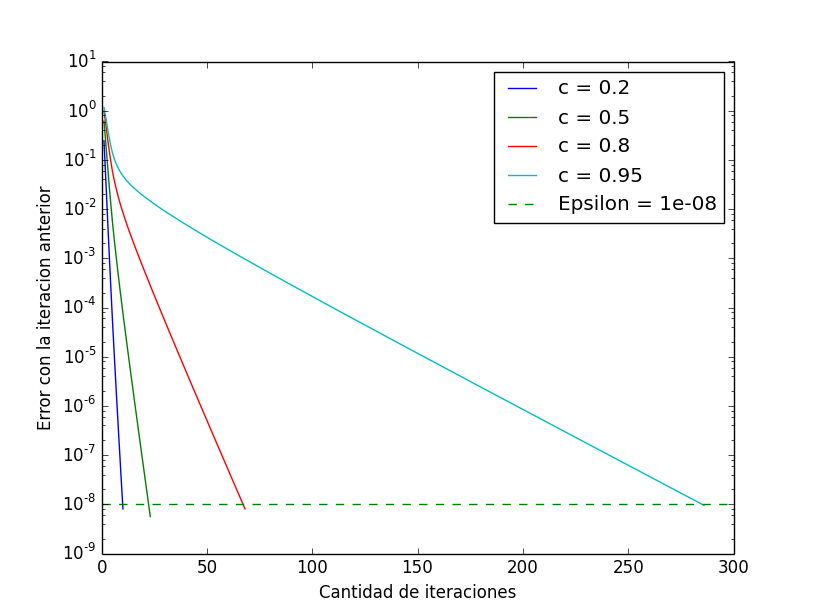
\includegraphics[width=0.9\textwidth]{errorSinQE.png}
    \caption{Evolución del error a lo largo de las iteraciones, sin QE}
    \label{}
\end{figure}

\begin{figure}[H]
  \centering
    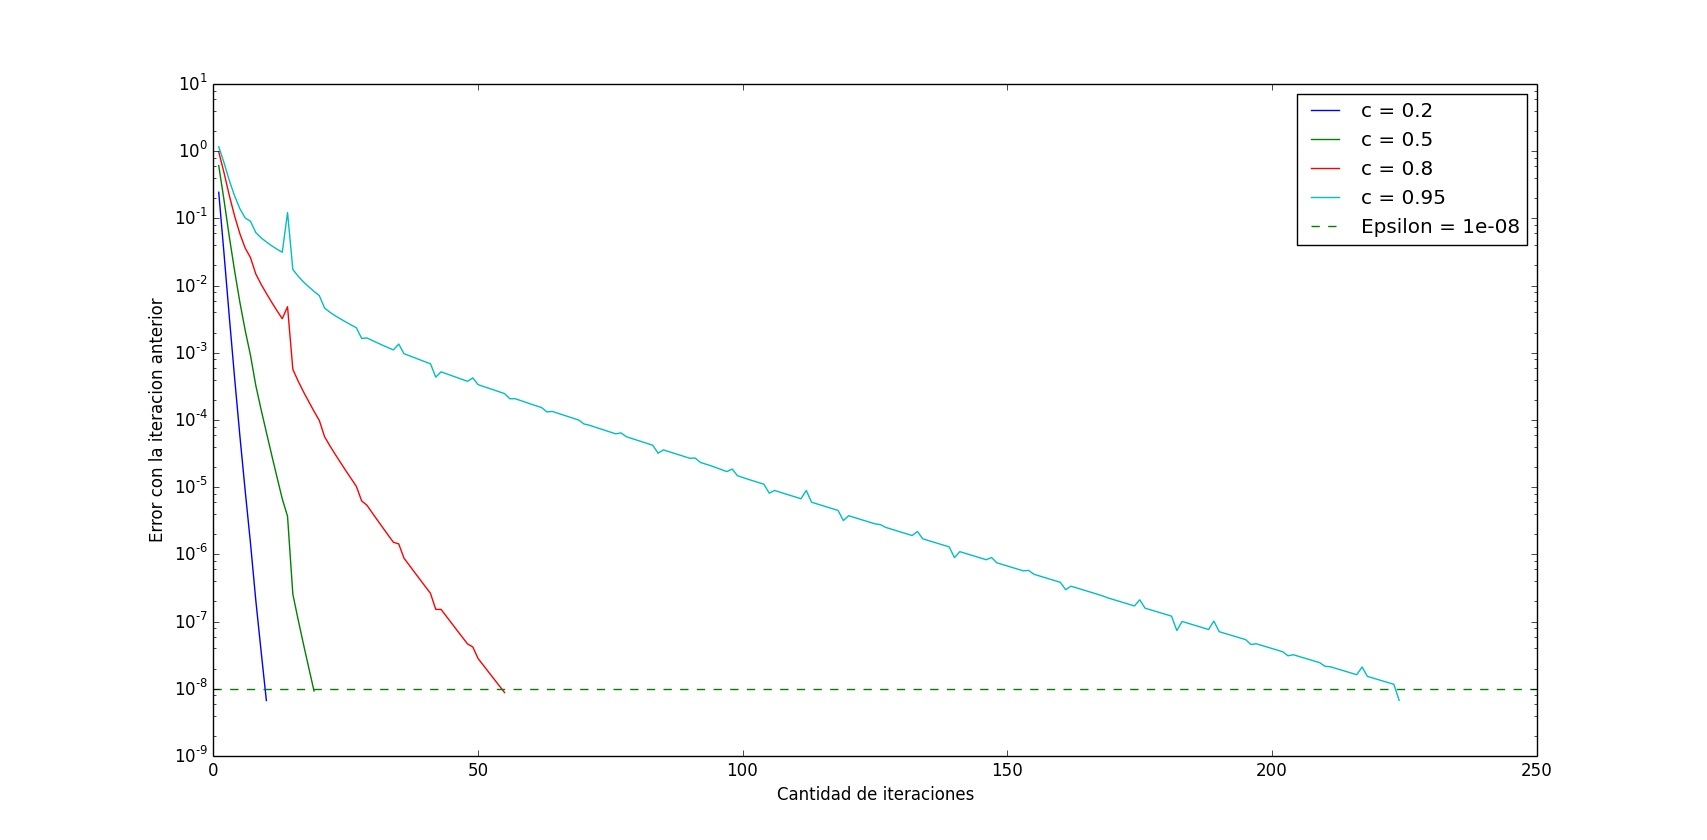
\includegraphics[width=0.9\textwidth]{errorConQE.png}
    \caption{Evolución del error a lo largo de las iteracions, con QE cada 7 iteraciones}
    \label{graf:errorQE}
\end{figure}

El m\'etodo de extrapolaci\'on se aplica cada 7 iteraciones, en el gr\'afico anterior (Fig. \ref{graf:errorQE}) se puede ver que se presentan picos m\'inimos y m\'aximos, esto se debe a que el m\'etodo previamente nombrado intenta operar con la combinación lineal de los autovectores que está generando el vector de la iteración en cuestión: minimizar los coeficientes de los autovectores no principales. Esto no necesariamente debería producir una aproximación mejor al autovector buscado, sino que genera condiciones más favorables para la convergencia del método de la potencia.

Se puede obvservar en las figuras que cuanto menor es el valor de $c$, m\'as r\'apido converge
el m\'etodo.  En estas circunstancias se otorga mayor importancia a la matriz uniforme $\left[\frac{1}{n}\right]$, cuyos autovalores son $1$ (dimensión $1$) y $0$ (dimensión $n-1$). Esta diferencia notable entre los autovalores favorece la convergencia del método de la potencia.\\

La diferencia que se da al utilizar extrapolaci\'on no se ve f\'acilmente en los gr\'aficos anteriores, por lo que vamos a mostrarlo con mas detalle:

\begin{figure}[H]
  \centering
    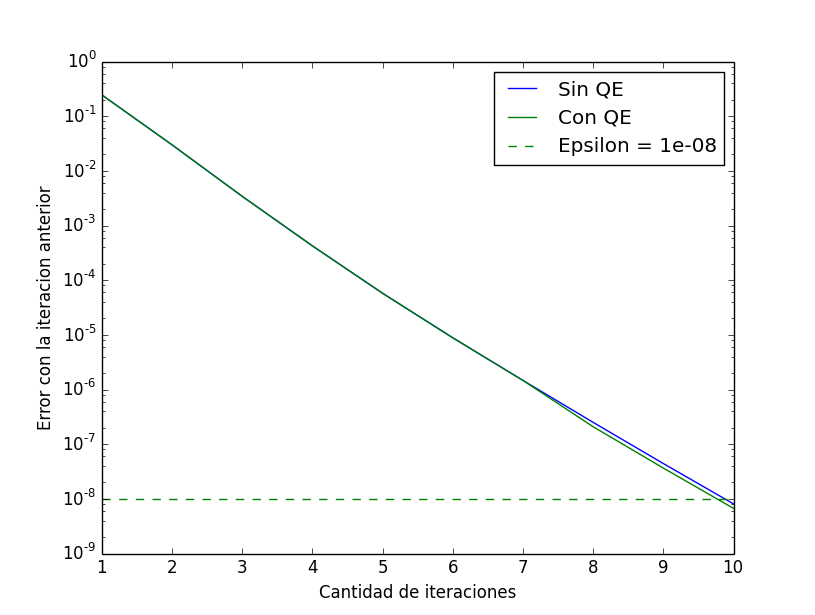
\includegraphics[width=0.8\textwidth]{comparando2.png}
    \caption{Comparaci\'on del uso de QE con $ c = 0.2$}
    \label{}
\end{figure}

\begin{figure}[H]
  \centering
    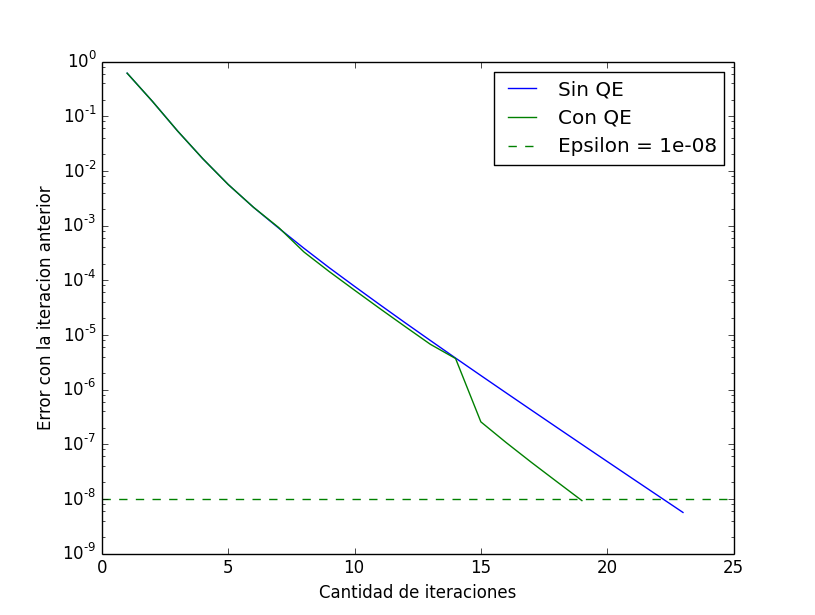
\includegraphics[width=0.8\textwidth]{comparando5.png}
    \caption{Comparaci\'on del uso de QE con $c = 0.5$}
    \label{}
\end{figure}

\begin{figure}[H]
  \centering
    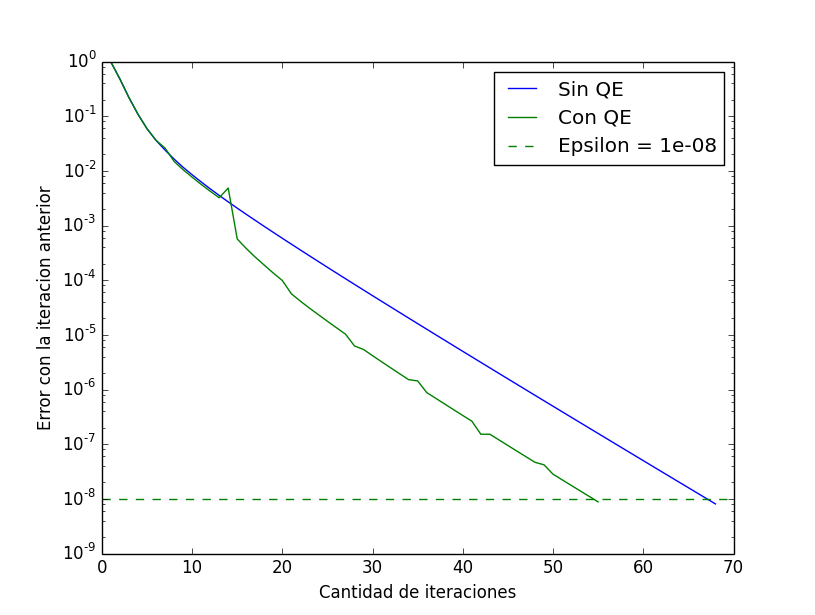
\includegraphics[width=0.8\textwidth]{comparando8.png}
    \caption{Comparaci\'on uso de QE con c = 0.8}
    \label{}
\end{figure}

\begin{figure}[H]
  \centering
    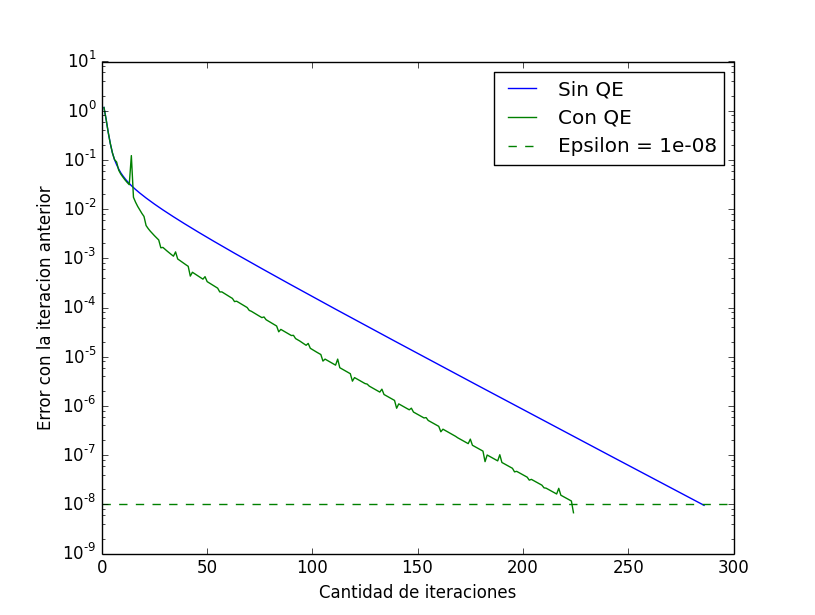
\includegraphics[width=0.8\textwidth]{comparando95.png}
    \caption{Comparaci\'on uso de QE con c = 0.95}
    \label{}
\end{figure}

En los gr\'aficos anteriores se nota la gran diferencia que hay cuando se aplica el m\'etodo de extrapolaci\'on cuadr\'atica, el cu\'al parece aumentar el error al principio, pero luego converge m\'as r\'apidamente. La diferencia tal vez no se aprecia tanto si la convergencia es muy r\'apida, como en el primer gr\'afico donde $c$ es igual a $0.2$, pero a medida que aumenta la cantidad de iteraciones, más conveniente es utilizarlo. Como dijimos antes, $c = 0.2$ ya provee una situación suficientemente buena para la convergencia del método de la potencia.\\


\subsection{Tiempo de ejecuci\'on}

Primero medimos tiempos de ejecuci\'on para distintos valores de $c$, aplicando o no QE, cada 7 iteraciones. Aquí notamos, que a pesar de la cantidad de iteraciones utilizando QE es menor, el m\'etodo de la potencia sin QE converge en menos tiempo de procesamiento (aunque no notablemente). Esto se debe a que realizar la extrapolación implica un tiempo extra de cómputo además de la iteración del método de la potencia, con lo cual, en casos donde éste converge rápidamente, agregar pasos de QE, si bien reduce la cantidad de iteraciones, implica un overhead que no resulta despreciable respecto del tiempo insumido por el algoritmo base. Para ajustar este costo, realizamos nuevas mediciones tomando el caso de mayor cantidad de iteraciones ($c = 0.95$) y variando la periodicidad con la que se aplica el método de extrapolación cuadrática.

A continuación mostramos las tablas de los valores obtenidos para esta experimentación, que puede ser reproducida siguiendo las instrucciones que se encuentran en el README.

Estos son los resultados arrojados por el algoritmo, primero con periodicidad de QE cada 7 iteraciones (Cuadro \ref{tab:tiempo}), y luego para el caso particular de $c = 0.95$ con periodicidad variable (Cuadro \ref{tab:pQE}). Como aclaración de la segunda tabla, $pQE$ hace referencia a la periodicidad con la que aplicamos QE en cantidad de iteraciones: \\
\begin{table}[H]
\centering
\begin{tabular}{ l | c | r}
  & Sin QE & Con QE\\
  \hline
  c = 0.2 & 2 segs. & 3 segs.\\
  \hline
  c = 0.5 & 6 segs. & 5 segs.\\
  \hline
  c = 0.8 & 15 segs. & 16 segs. \\
  \hline
  c = 0.95 & 65 segs. & 69 segs. \\
  \hline
\end{tabular}
\caption{Tiempo de ejecución para distintos valores de $c$, aplicando o no QE.}
\label{tab:tiempo}
\end{table}
 Como dijimos, el cuadro \ref{tab:tiempo} muestra que el tiempo de ejecución  aplicando QE cada 7 iteraciones del algoritmo es mayor que el que no lo utiliza.

\begin{table}
\centering
\begin{tabular}{ l | c | c}
  & Tiempo de ejecución & Cantidad de iteraciones\\
  \hline
  pQE = 5 & 78 segs. & 229 iters.\\
  \hline
  pQE = 20 & 59 segs. & 225 iters.\\
  \hline
  pQE = 35 & 54 segs. & 218 iters. \\
  \hline
  pQE = 50 & 52 segs. & 213 iters. \\
  \hline
  pQE = 65 & 52 segs. & 218 iters. \\
  \hline
  pQE = 70 & 53 segs. & 219 iters. \\
  \hline
  pQE = 90 & 52 segs. & 222 iters. \\
  \hline
  pQE = 105 & 52 segs. & 221 iters. \\
  \hline
  pQE = 120 & 57 segs. & 240 iters. \\
  \hline
  pQE = 135 & 57 segs. & 241 iters. \\
  \hline
\end{tabular}
\caption{Tiempo de ejecución y cantidad de iteraciones para la aplicación de QE con distinta periodicidad, $c = 0.95$.}
\label{tab:pQE}
\end{table}
Como podemos observar el cuadro \ref{tab:tiempo}, lo que suponíamos es un hecho: variar el momento en que se aplica el método de extrapolación cuadrática así como también la cantidad de veces que se aplica, ayuda a acelerar aún más la velocidad de convergencia del método de la potencia estándar. Es interesante apreciar asimismo, que aún teniendo el mismo tiempo de ejecución para algunos valores de $pQE$, la cantidad de iteraciones es distinta y esto se debe a que variar el momento en que se aplica QE, y no sólo la cantidad de veces que se aplica es un factor a tener en cuenta. Queda pendiente esta experimentación, la cual es determinar la estrategia más conveniente a la hora de distribuir la aplicación de QE, es decir, ¿conviene aplicar el método cada cierta cantidad de iteraciones fija, de manera uniforme, o dependiendo de otros factores?

Como última observación, el mejor resultado se obtuvo con una periodicidad de 50 iteraciones, donde QE fue aplicado 4 veces logrando cantidad de iteraciones mínima al igual que tiempo de ejecución mínimo, contrastando contra todo los otros resultados obtenidos (recordemos del cuadro \ref{tab:tiempo}, que el tiempo de ejecución sin QE para esta situación es de 65 segundos, valor que es mayor que todos los listados en la tabla \ref{tab:pQE}).

\subsection{Relevancia de las p\'aginas}

A continuación incluimos un ejemplo reducido para observar cómo funciona efectivamente el ranking mediante este algoritmo. A partir del script proporcionado por la cátedra, construimos el grafo de conectividad para algunas páginas con links entre sí (de diferentes diarios y medios) y otras de interés general o de computación que no están apuntadas por éstas. En el cuadro \ref{tab:ranking} presentamos el ordenamiento obtenido, para los cuatro valores de $c$ con los que trabajamos anteriormente.
\begin{table}\begin{center}
\subfloat[][Rank obtenido con $c = 0.2$]{\begin{tabular}{ l | c }
  \hline
www.ole.com.ar & 0.0484629 \\
www.clarin.com & 0.0468603 \\
www.ciudad.com.ar & 0.0430782 \\
www.clasificados.clarin.com & 0.0430782 \\
\textbf{www.youtube.com} & 0.0420166 \\
www.taringa.net & 0.0420166 \\
canchallena.lanacion.com.ar & 0.0418644 \\
www.lanacion.com.ar & 0.0418644 \\
www.zonaprop.com.ar & 0.0405957 \\
www.rollingstone.com.ar & 0.0405957 \\
maps.google.com.ar & 0.0385152 \\
www.twitter.com & 0.0385152 \\
\textbf{www.clarin.com/deportes} & 0.0373568 \\
www.9gag.com & 0.0350138 \\
www.stackoverflow.com & 0.0350138 \\
www.facebook.com & 0.0350138 \\
www.hotmail.com & 0.0350138 \\
www.gmail.com & 0.0350138 \\
www.assembla.com & 0.0350138 \\
www.github.com & 0.0350138 \\
www.mercadolibre.com.ar & 0.0350138 \\
www.yahoo.com & 0.0350138 \\
www.pagina12.com.ar & 0.0350138 \\
www.mamapuntocero.com.ar & 0.0350138 \\
www.infobae.com & 0.0350138 \\
www.google.com & 0.0350138 \\
  \hline
\end{tabular}
}
\qquad
\subfloat[][Rank obtenido con $c = 0.5$]{
\begin{tabular}{ l | c }
  \hline
www.ole.com.ar & 0.0708548 \\
www.clarin.com & 0.0679806 \\
www.ciudad.com.ar & 0.0551093 \\
www.clasificados.clarin.com & 0.0551093 \\
canchallena.lanacion.com.ar & 0.0476948 \\
www.lanacion.com.ar & 0.0476948 \\
www.zonaprop.com.ar & 0.0445151 \\
www.rollingstone.com.ar & 0.0445151 \\
\textbf{www.youtube.com} & 0.0429253 \\
www.taringa.net & 0.0429253 \\
\textbf{www.clarin.com/deportes} & 0.0371144 \\
maps.google.com.ar & 0.0357711 \\
www.twitter.com & 0.0357711 \\
www.9gag.com & 0.0286169 \\
www.stackoverflow.com & 0.0286169 \\
www.facebook.com & 0.0286169 \\
www.hotmail.com & 0.0286169 \\
www.gmail.com & 0.0286169 \\
www.assembla.com & 0.0286169 \\
www.github.com & 0.0286169 \\
www.mercadolibre.com.ar & 0.0286169 \\
www.yahoo.com & 0.0286169 \\
www.pagina12.com.ar & 0.0286169 \\
www.mamapuntocero.com.ar & 0.0286169 \\
www.infobae.com & 0.0286169 \\
www.google.com & 0.0286169 \\
\hline
\end{tabular}
}
\\ 
\vspace{0.5cm}
\subfloat[][Rank obtenido con $c = 0.8$]{\begin{tabular}{ l | c }
  \hline
www.ole.com.ar & 0.122585 \\
www.clarin.com & 0.119996 \\
www.ciudad.com.ar & 0.0862634 \\
www.clasificados.clarin.com & 0.0862634 \\
canchallena.lanacion.com.ar & 0.0492588 \\
www.lanacion.com.ar & 0.0492588 \\
www.zonaprop.com.ar & 0.0445675 \\
www.rollingstone.com.ar & 0.0445675 \\
\textbf{www.clarin.com/deportes} & 0.0422953 \\
\textbf{www.youtube.com} & 0.032933 \\
www.taringa.net & 0.032933 \\
maps.google.com.ar & 0.0256146 \\
www.twitter.com & 0.0256146 \\
www.9gag.com & 0.0182961 \\
www.stackoverflow.com & 0.0182961 \\
www.facebook.com & 0.0182961 \\
www.hotmail.com & 0.0182961 \\
www.gmail.com & 0.0182961 \\
www.assembla.com & 0.0182961 \\
www.github.com & 0.0182961 \\
www.mercadolibre.com.ar & 0.0182961 \\
www.yahoo.com & 0.0182961 \\
www.pagina12.com.ar & 0.0182961 \\
www.mamapuntocero.com.ar & 0.0182961 \\
www.infobae.com & 0.0182961 \\
www.google.com & 0.0182961 \\
  \hline
\end{tabular}
}
\qquad
\subfloat[][Rank obtenido con $c = 0.95$]{
\begin{tabular}{ l | c }
  \hline
www.ole.com.ar & 0.205635 \\
www.clarin.com & 0.204461 \\
www.ciudad.com.ar & 0.138847 \\
www.clasificados.clarin.com & 0.138847 \\
\textbf{www.clarin.com/deportes} & 0.0559973 \\
canchallena.lanacion.com.ar & 0.028682 \\
www.lanacion.com.ar & 0.028682 \\
www.zonaprop.com.ar & 0.0256032 \\
www.rollingstone.com.ar & 0.0256032 \\
\textbf{www.youtube.com} & 0.0145039 \\
www.taringa.net & 0.0145039 \\
maps.google.com.ar & 0.0109709 \\
www.twitter.com & 0.0109709 \\
www.9gag.com & 0.00743788 \\
www.stackoverflow.com & 0.00743788 \\
www.facebook.com & 0.00743788 \\
www.hotmail.com & 0.00743788 \\
www.gmail.com & 0.00743788 \\
www.assembla.com & 0.00743788 \\
www.github.com & 0.00743788 \\
www.mercadolibre.com.ar & 0.00743788 \\
www.yahoo.com & 0.00743788 \\
www.pagina12.com.ar & 0.00743788 \\
www.mamapuntocero.com.ar & 0.00743788 \\
www.infobae.com & 0.00743788 \\
www.google.com & 0.00743788 \\
\hline
\end{tabular}
}

\caption{Rank obtenido para distintos valores de $c$}
\label{tab:ranking}
\end{center}\end{table}

Tal como esper\'abamos ver, las 15 p\'aginas que hab\'iamos notado que no ten\'ian links entrantes, son las \'ultimas
en la tabla, independientemente del valor de $c$ y, no casualmente, tienen todas la misma relevancia.

También se observa que a medida que el valor de $c$ aumenta, y por ende, el comportamiento aleatorio tiene menos preponderancia, se agrupan al principio las páginas que efectivamente guardan relación cercana (Olé, Clarín y sus secciones, Ciudad, La Nación, etc), mientras que páginas más generales como YouTube o Taringa pierden importancia. Resaltamos para ejemplificar esto clarin/deportes y YouTube. Pensando en una web exclusivamente compuesta por estas páginas esta situación tiene sentido: un portal de videos es menos relevante que una página de deportes, dado que buena parte de los enlaces existentes en esta red están dedicados a noticias.

